\section{Opis algorytmu}
Zadaniem programu jest pokolorowanie wierzchołków zadanego grafu z użyciem jak najmniejszej liczby kolorów.
Kolorowanie odbywa się z wykorzystaniem heurystycznego algorytmu przeszukiwania z tabu.
Węzłem przestrzeni przeszukiwań jest pokolorowany (legalnie bądź nie) graf.

\subsection{Funckja celu}
Algorytm dąży do minimalizacji funkcji celu\footnote{Definicja funkcji celu zaczerpnięta z: D. S. Johnson, C. R. Aragon, L. A. McGeoch, C. Schevon, Optimization by Simulated Annealing: An Experimental Evaluation; Part II, Graph Coloring and Number Partitioning, Operations Research, Vol. 39, No. 3, May-June 1991, pp. 378-406.}:

\begin{equation}
 f(G) = -\sum_{i=1}^{k} C_i^2 + \sum_{i=1}^{k} 2 C_i E_i
\end{equation}

gdzie:
\begin{itemize}
 \item $G$ - graf, dla którego liczona jest funkcja celu,
 \item $k$ - liczba kolorów użytych do pokolorowania grafu $G$,
 \item $C_i$ - liczba wierzchołków grafu $G$ pokolorowanych na $i$-ty kolor,
 \item $E_i$ - liczba krawędzi grafu $G$, których oba końce pokolorowane są na $i$-ty kolor.
\end{itemize}

Definicję funkcji należy rozumieć następująco:

\begin{enumerate}
 \item z jednej strony, faworyzowane są pokolorowania z użyciem jak najmniejszej liczby kolorów,
 \item z drugiej strony, dyskryminowane są pokolorowania nielegalne.
\end{enumerate}

\subsection{Lista tabu}
Lista tabu zawiera ograniczoną liczbę ostatnich akcji podjętych przez algorytm.
Pojedynczą akcją jest pokolorowanie pojedycznego wierzchołka na określony kolor.

\subsection{Przykład}

Graf:

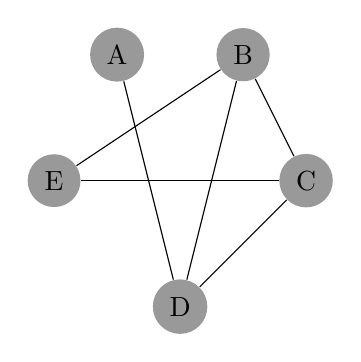
\begin{tikzpicture}
  [scale=.8,auto=left,
   every node/.style={circle,fill=black!40},
   0/.style={fill=red!50},
   1/.style={fill=blue!50},
   2/.style={fill=green!50},
   3/.style={fill=yellow!50},
   4/.style={fill=purple!50}]
  
  \node (A) at (2,4) {A};
  \node (B) at (4,4) {B};
  \node (C) at (5,2) {C};
  \node (D) at (3,0) {D};
  \node (E) at (1,2) {E};

  \foreach \from/\to in {A/D,B/C,B/E,C/E,D/B,C/D}
    \draw (\from) -- (\to);
\end{tikzpicture}



\subsubsection{Krok 0}

Graf:

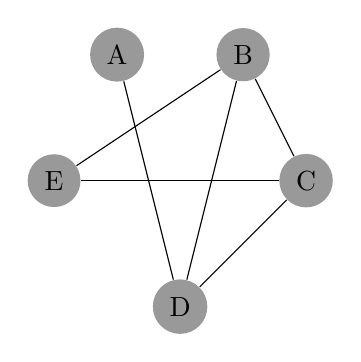
\begin{tikzpicture}
  [scale=.8,auto=left,
   every node/.style={circle,fill=black!40},
   0/.style={fill=red!50},
   1/.style={fill=blue!50},
   2/.style={fill=green!50},
   3/.style={fill=yellow!50},
   4/.style={fill=purple!50}]
  
  \node (A) at (2,4) {A};
  \node (B) at (4,4) {B};
  \node (C) at (5,2) {C};
  \node (D) at (3,0) {D};
  \node (E) at (1,2) {E};

  \foreach \from/\to in {A/D,B/C,B/E,C/E,D/B,C/D}
    \draw (\from) -- (\to);
\end{tikzpicture}

Lista tabu jest pusta.



\subsubsection{Krok 1}

Graf:

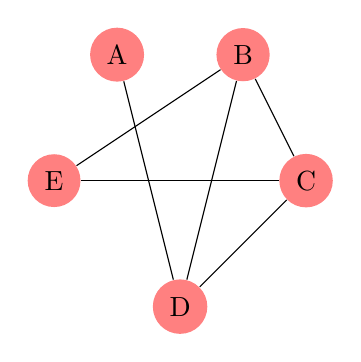
\begin{tikzpicture}
  [scale=.8,auto=left,
   every node/.style={circle,fill=black!40},
   0/.style={fill=red!50},
   1/.style={fill=blue!50},
   2/.style={fill=green!50},
   3/.style={fill=yellow!50},
   4/.style={fill=purple!50}]
  
  \node [0] (A) at (2,4) {A};
  \node [0] (B) at (4,4) {B};
  \node [0] (C) at (5,2) {C};
  \node [0] (D) at (3,0) {D};
  \node [0] (E) at (1,2) {E};

  \foreach \from/\to in {A/D,B/C,B/E,C/E,D/B,C/D}
    \draw (\from) -- (\to);
\end{tikzpicture}

Lista tabu:

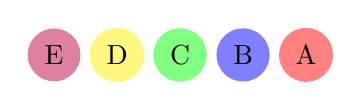
\begin{tikzpicture}
  [scale=.8,auto=left,
   every node/.style={circle,fill=black!40},
   0/.style={fill=red!50},
   1/.style={fill=blue!50},
   2/.style={fill=green!50},
   3/.style={fill=yellow!50},
   4/.style={fill=purple!50}]
  
  \node [0] (A) at (0,0) {A};
  \node [1] (B) at (-1,0) {B};
  \node [2] (C) at (-2,0) {C};
  \node [3] (D) at (-3,0) {D};
  \node [4] (E) at (-4,0) {E};
\end{tikzpicture}